%\begin{figure}[htbp]
%  \centering
%  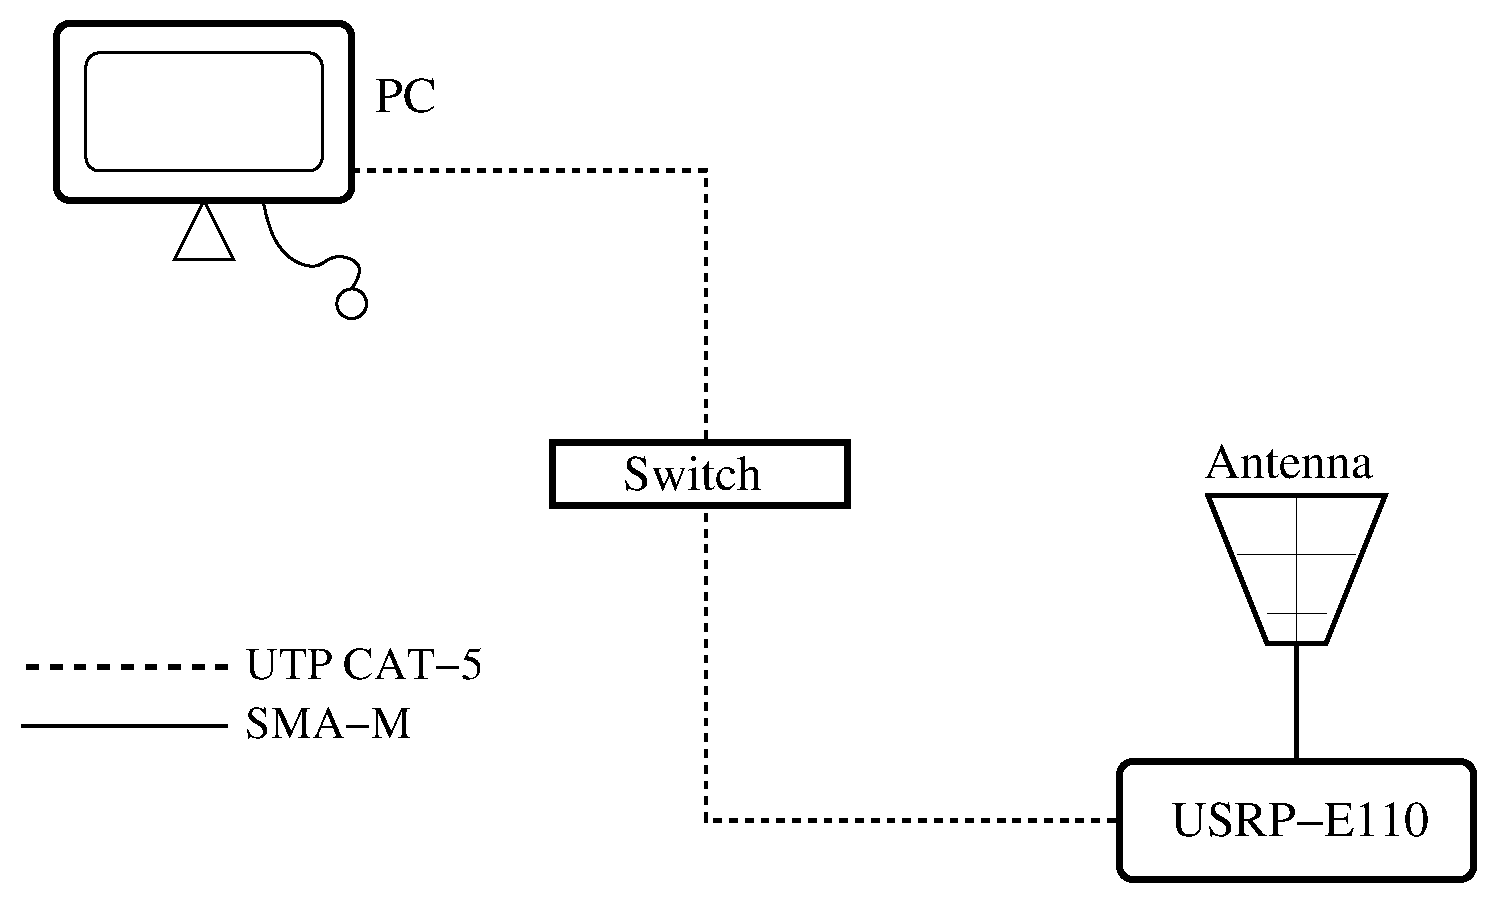
\includegraphics[width = 3cm]{sect2/figures/example_to_be_removed.eps}
%  \caption{TODO remove.}
%  \label{fig:example}
%\end{figure}

\subsection{Pilot's deployments}

This section presents the optical fibre (OF) deployments from the Points-Of-Presence (POPs) to the end users. Therefore it mainly refers to the physical wire deployment. The POPs are described in section~\ref{pops}.

\subsubsection{Gurb}

TODO

\subsubsection{Vic}




\subsubsection{Rub\'{i}}

Rub\'{i} local government in early 2012 showed interest in deploying fiber following a Bottom-up Broadband model.
The first goal was to offer high-speed Internet connections to the largest companies operating in one of Rub\'{i}'s industrial areas called ''Can Jardi''.
These companies had access only to slow ADSL connections and the absence of a fiber deployment was seriously affecting their competitiveness.
The lack of commercial high speed connections offering prompted the city's local government to look for alternatives.

An initial round of conversations took place in Spring 2012 to plan for a deployment during the Summer.
The planning involved a strong participation of a local partner, company with experience in wireless BuB deployment.
This initial planning for a bottom-up-broadband deployment did not pass unnoticed, and commercial ISPs approached the Rub\'{i} local government with fiber deployment offerings.
The offering was to place the city of Rub\'{i} high in de ISPs fiber deployment plans and prioritize it over other cities.
Guifi, UPF and the local partner were asked by the city's local government to prepare a concrete offering that could match the offering of the ISPs.

The arrival of traditional ISPs proposals, combined with the uncertainties of the competence of the local partner to carry out fiber deployments and internal discrepancies in the Rub\'{i}'s local government slowed down the pilot.
Currently this pilot is on hold, and it is not clear how it will resolve.
Personal interests and personal connections within the City Hall may play an important role in the final resolution.

It is remarkable that the fact that the City Hall entered in conversations to plan a BuB deployment triggered a number of events that placed the city in a much favourable situation to negotiate with the ISPs about future fiber deployments.

\subsection{Other deployments}

